\documentclass[slides,compress]{beamer}
\usepackage{graphicx,amsmath,hyperref}
\usepackage{verbatim}

\usepackage[normalem]{ulem}

\usetheme{default}
\useinnertheme{rectangles}

\title{{\huge You can't get the staff - an electronic alternative...}}

\author{Graeme Winter}
\institute{Diamond Light Source}
\date{CCP4 Study Weekend 2012}

\begin{document}

\setbeamertemplate{background}{

\includegraphics[width=\paperwidth,height=\paperheight]
{diamond-background.png}
}

\frame{\maketitle}

\frame{
\frametitle{Overview}
\begin{itemize}
\item{Background}
\item{What is xia2?}
\item{What does it do and how do I use it?}

\end{itemize}
}

\section{Background}

\begin{frame}
\frametitle{Before we start...}
\begin{itemize}
\uncover<1->{\item{No MOSFLM, XDS, SCALA, CCP4}}
\uncover<1->{\item{$\rightarrow$ no xia2}}
\uncover<2->{\item{No LABELIT, CCTBX, POINTLESS etc.}}
\uncover<2->{\item{$\rightarrow$ harder to write xia2, less reliable}}
\end{itemize}
\end{frame}

\begin{frame}
\frametitle{Acknowledgements}
\begin{itemize}
\item{Andrew Leslie, Harry Powell, Phil Evans, Wolfgang Kabsch, Kay Diederichs,
Nick Sauter, Ralf Grosse-Kunstleve}
\item{Alun Ashton, Dave Stuart, Diamond beamline staff, Miroslav Papiz, 
Steve Prince, Colin Nave, xia2 users, providers of test data (esp. JCSG)}
\end{itemize}
\end{frame}

\begin{frame}
\frametitle{Background}
\begin{itemize}
\uncover<1->{
\item{Comprehensive, trusted software available}
\item{Background of strong publications (esp. CCP4 study weekends)}
\item{Massive advances in computing}
\item{New synchrotron for UK}
}
\uncover<2->{
\item{$\rightarrow$ a great time to develop automated data reduction}
}
\end{itemize}
\end{frame}

\section{What is xia2?}
\begin{frame}
\frametitle{What is xia2?}
{\large
\uncover<1->{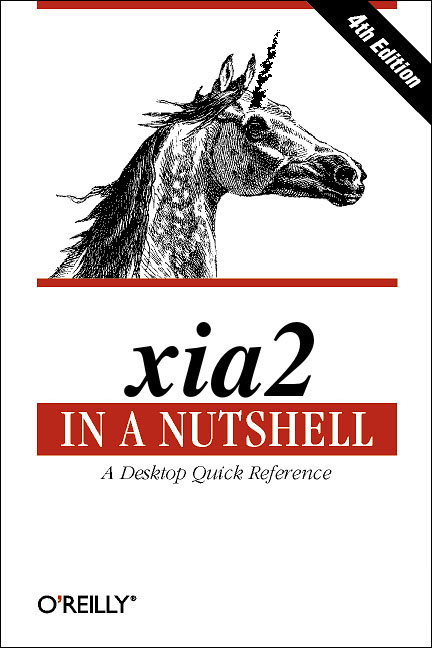
\includegraphics[scale=0.125]{figures/xia2-in-a-nutshell.jpg}}
\uncover<2->{
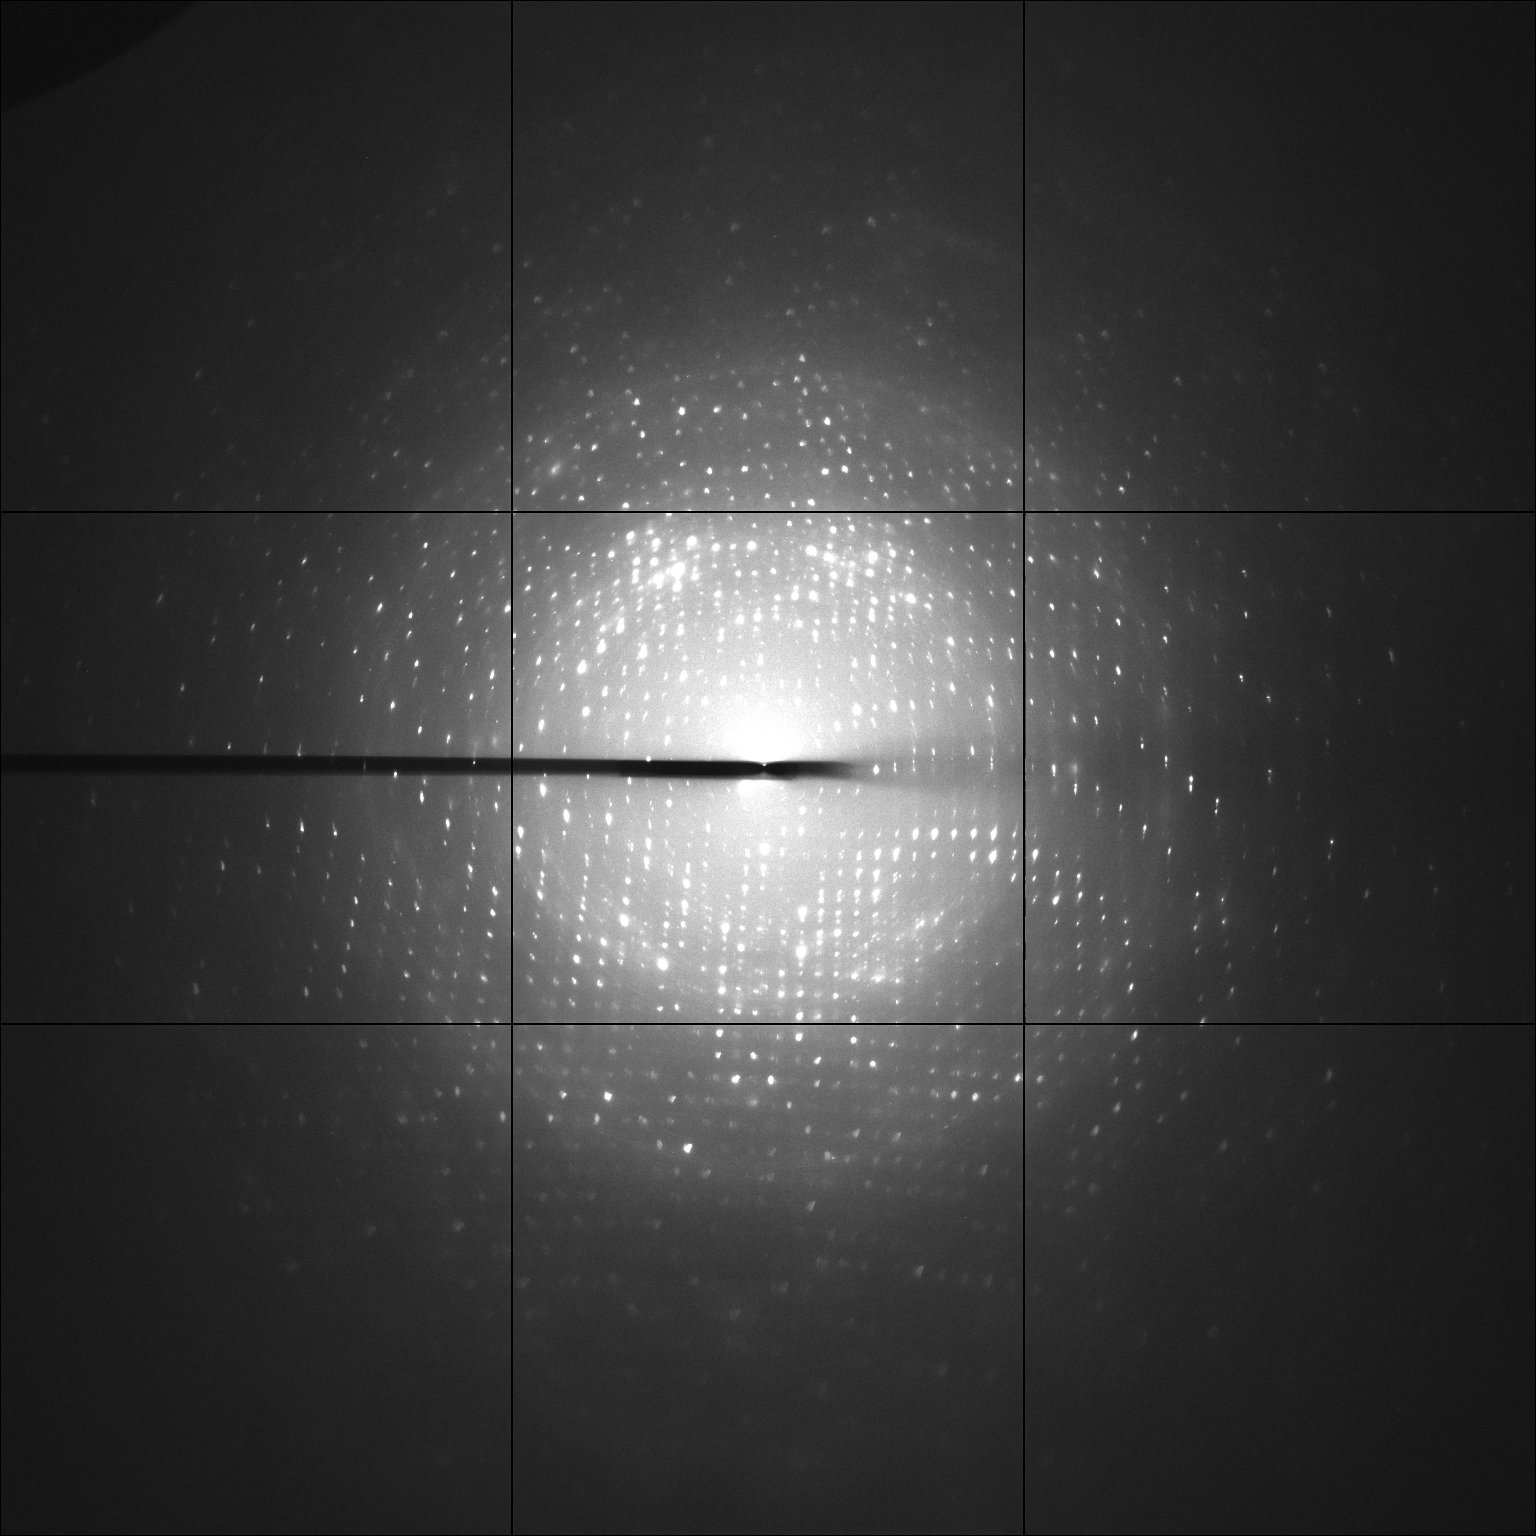
\includegraphics[scale=0.05]{figures/example-diffraction-image-small.jpg} 
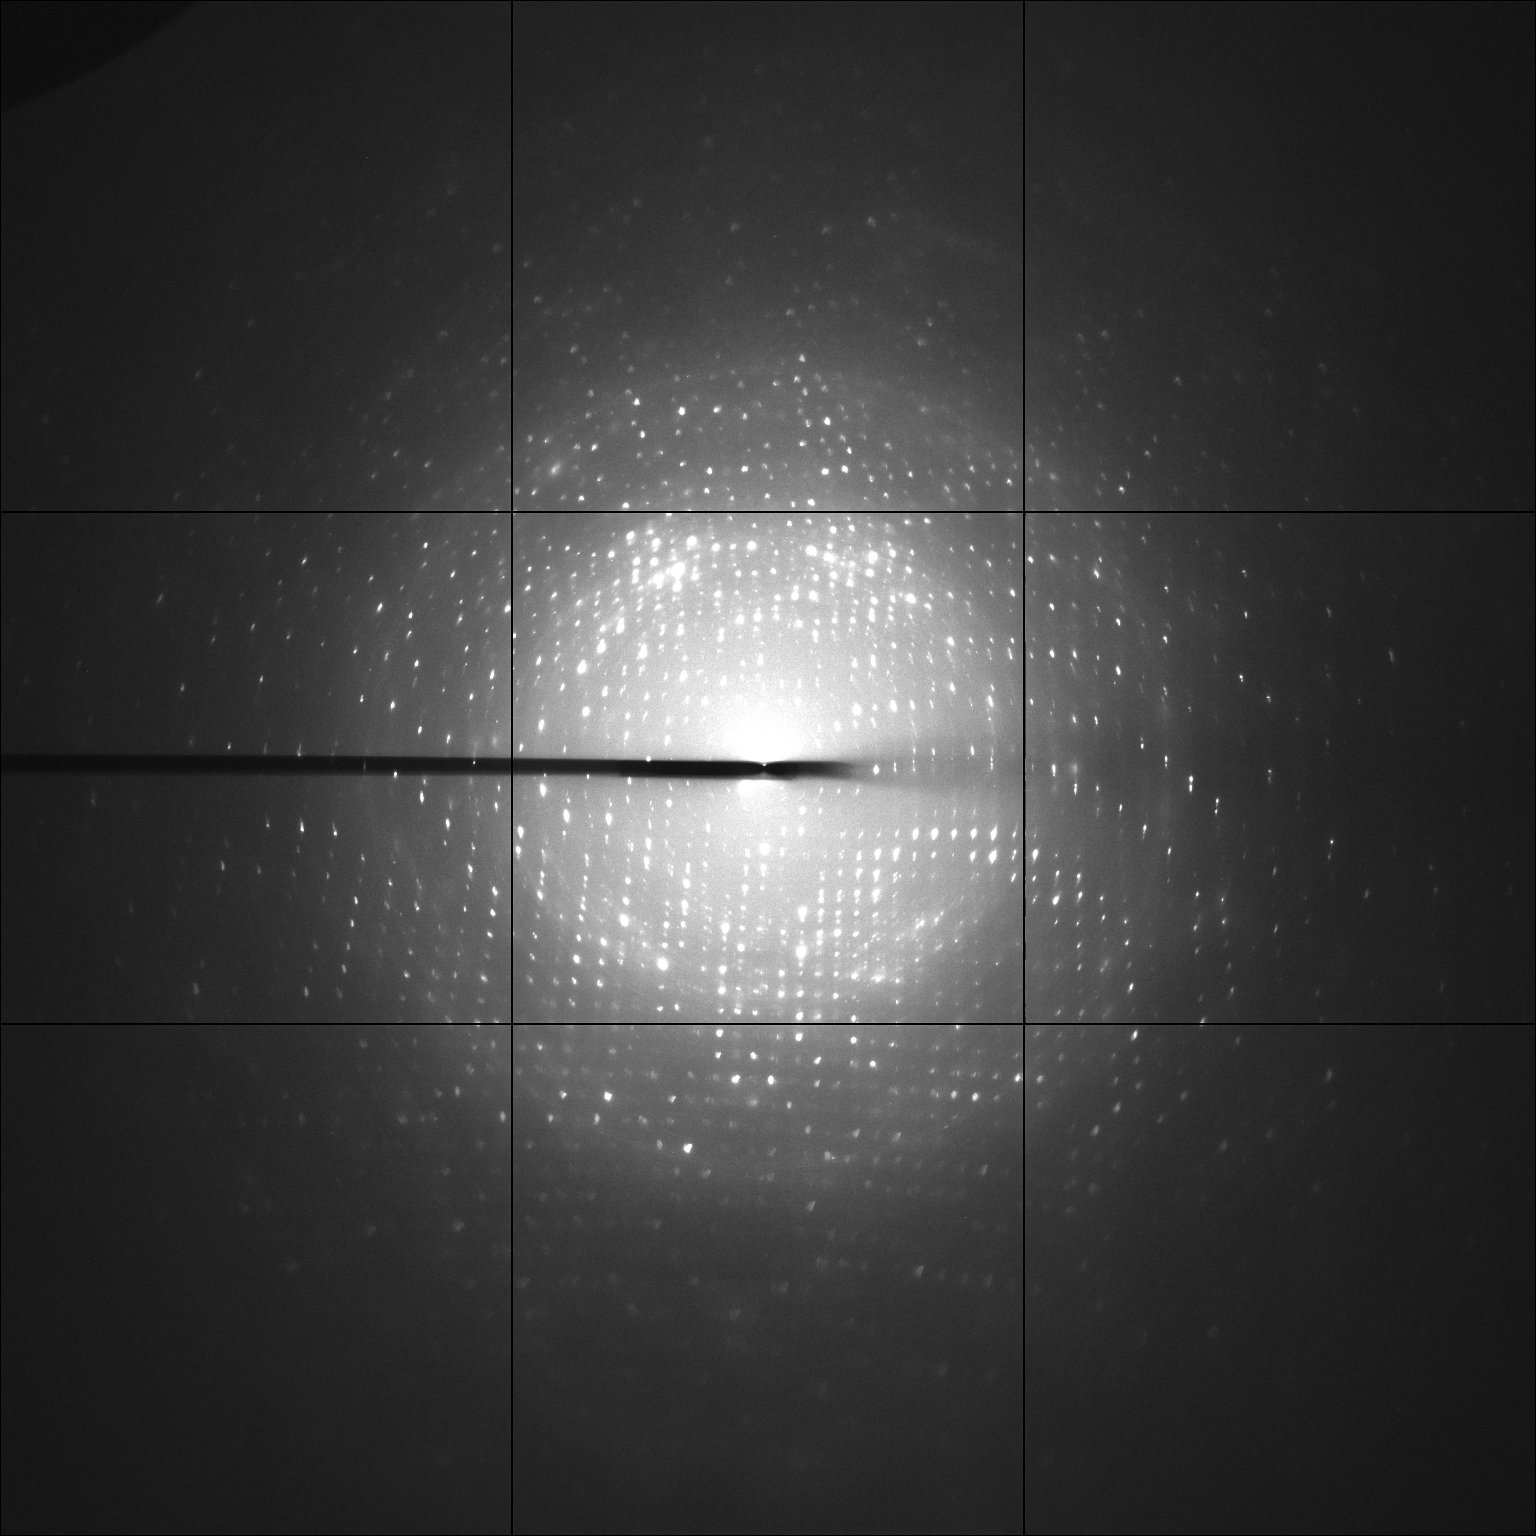
\includegraphics[scale=0.05]{figures/example-diffraction-image-small.jpg}
}
\uncover<3->{$\rightarrow H K L I \sigma_{I}$}
}
\end{frame}

\begin{frame}
\frametitle{What is xia2?}
\begin{itemize}
\uncover<1->{
\item{An \emph{expert} system to perform diffraction data and processing on 
your behalf using your software}
}
\uncover<2->{
\item{A system which can correctly handle multi-pass, multi-wavelength data
sets}
}
\uncover<3->{
\item{\emph{Not} a data processing package}
}
\end{itemize}
\end{frame}

\begin{frame}
\frametitle{Why ``you can't get the staff?''}
\begin{itemize}
\item{12 datasets / hour possible}
\item{Limited help}
\item{Human endurance}
\item{Intended xia2 as tool to delegate data processing to}
\end{itemize}
\end{frame}

\begin{frame}
\frametitle{Why is this useful?}
\begin{itemize}
\item{Second opinion}
\item{Allows you to focus on problem cases}
\item{Help  busy / novice users}
\item{Provides access to other tools}
\item{Reproducible processing}
\end{itemize}
\end{frame}

\begin{frame}
\frametitle{Using xia2}
%{\centerline
\begin{tabular}{c}
{\huge
xia2 -2d /here/are/my/data
}\\
\\
{\huge \emph{- or -}} \\
\\
{\huge
xia2 -3d /here/are/my/data
}\\
\end{tabular}
%}
\end{frame}


\end{document}
